\documentclass{article}
\usepackage{graphicx}
\usepackage{float}
\usepackage[export]{adjustbox}
\usepackage{tabularx}
\usepackage{multirow}
\usepackage{multicol}
\usepackage{booktabs}
\usepackage[table]{xcolor}
\usepackage{natbib}
\setcitestyle{round}

\title{Assignment 2, Replication and extension of Muchlinski et al. (2016)\\Random forest vs logistic regression}
\date{October 15, 2020}
\author{Eve Fleisig, Jordan Klein, Matthew Sun}

\begin{document}

\maketitle

\section*{Part 1: Replication}

We begin by replicating the separation plots from  \cite{muchlinski2016comparing}
using their updated replication materials (Fig.~\ref{fig:separation}). Our separation plots for the logistic regression models by Fearon and Laitin (2003), Collier and Hoeffler (2004), and Hegre and Sambanis (2006) are identical to those from Muchlinski et al's original paper, but notably, our separation plot for random forests identifies 2 false positives while that from Muchlinski et al's original paper does not identify any. These results align with those produced by Mulchinksi et al in their own replication \citep{muchlinski_2019}.

\begin{table}[H]
\centering
\caption{Predicted probability of civil war onset: Logistic Regression and Random Forests}
\resizebox{\linewidth}{!}{
    \begin{tabular}{lccccc}
    \toprule
    \multicolumn{6}{c}{Models and predicted probability of civil war onset} \\
    \cmidrule(l{3pt}r{3pt}){1-6}
Country & Year & Fearon and Latin (2003) & Collier and Hoeffler (2004) & Hegre and Sambanis (2006) & Random Forest\\
    \midrule
    \rowcolor{gray!6}  Afghanistan & 2001 & 0.01 & 0.00 & 0.00 & 0.06\\
Angola & 2001 & 0.01 & 0.01 & 0.02 & 0.71\\
    \rowcolor{gray!6}  Burundi & 2001 & 0.03 & 0.00 & 0.02 & 0.09\\
Guinea & 2001 & 0.01 & 0.00 & 0.01 & 0.07\\
    \rowcolor{gray!6}  Rwanda & 2001 & 0.01 & 0.00 & 0.01 & 0.05\\
\addlinespace
Uganda & 2002 & 0.02 & 0.02 & 0.02 & 0.93\\
    \rowcolor{gray!6}  Liberia & 2003 & 0.02 & 0.04 & 0.03 & 0.98\\
Iraq & 2004 & 0.03 & 0.01 & 0.03 & 0.16\\
    \rowcolor{gray!6}  Uganda & 2004 & 0.01 & 0.00 & 0.01 & 0.45\\
Afghanistan & 2005 & 0.03 & 0.00 & 0.02 & 0.14\\
    \addlinespace
    \rowcolor{gray!6}  Chad & 2006 & 0.02 & 0.04 & 0.03 & 0.98\\
Somalia & 2007 & 0.06 & 0.04 & 0.10 & 0.96\\
    \rowcolor{gray!6}  Rwanda & 2009 & 0.02 & 0.04 & 0.03 & 0.99\\
Libya & 2011 & 0.02 & 0.04 & 0.02 & 0.95\\
    \rowcolor{gray!6}  Syria & 2012 & 0.01 & 0.00 & 0.00 & \vphantom{1} 0.06\\
    \addlinespace
Syria & 2012 & 0.01 & 0.00 & 0.00 & 0.06\\
    \rowcolor{gray!6}  Democratic Republic of the Congo & 2013 & 0.01 & 0.00 & 0.00 & 0.04\\
Iraq & 2013 & 0.02 & 0.04 & 0.02 & 0.96\\
    \rowcolor{gray!6}  Nigeria & 2013 & 0.02 & 0.04 & 0.03 & 0.96\\
Somalia & 2014 & 0.05 & 0.04 & 0.11 & 0.99\\
    \bottomrule
\end{tabular}}
\end{table}

\begin{figure}[H]
     \makebox[\textwidth][c]{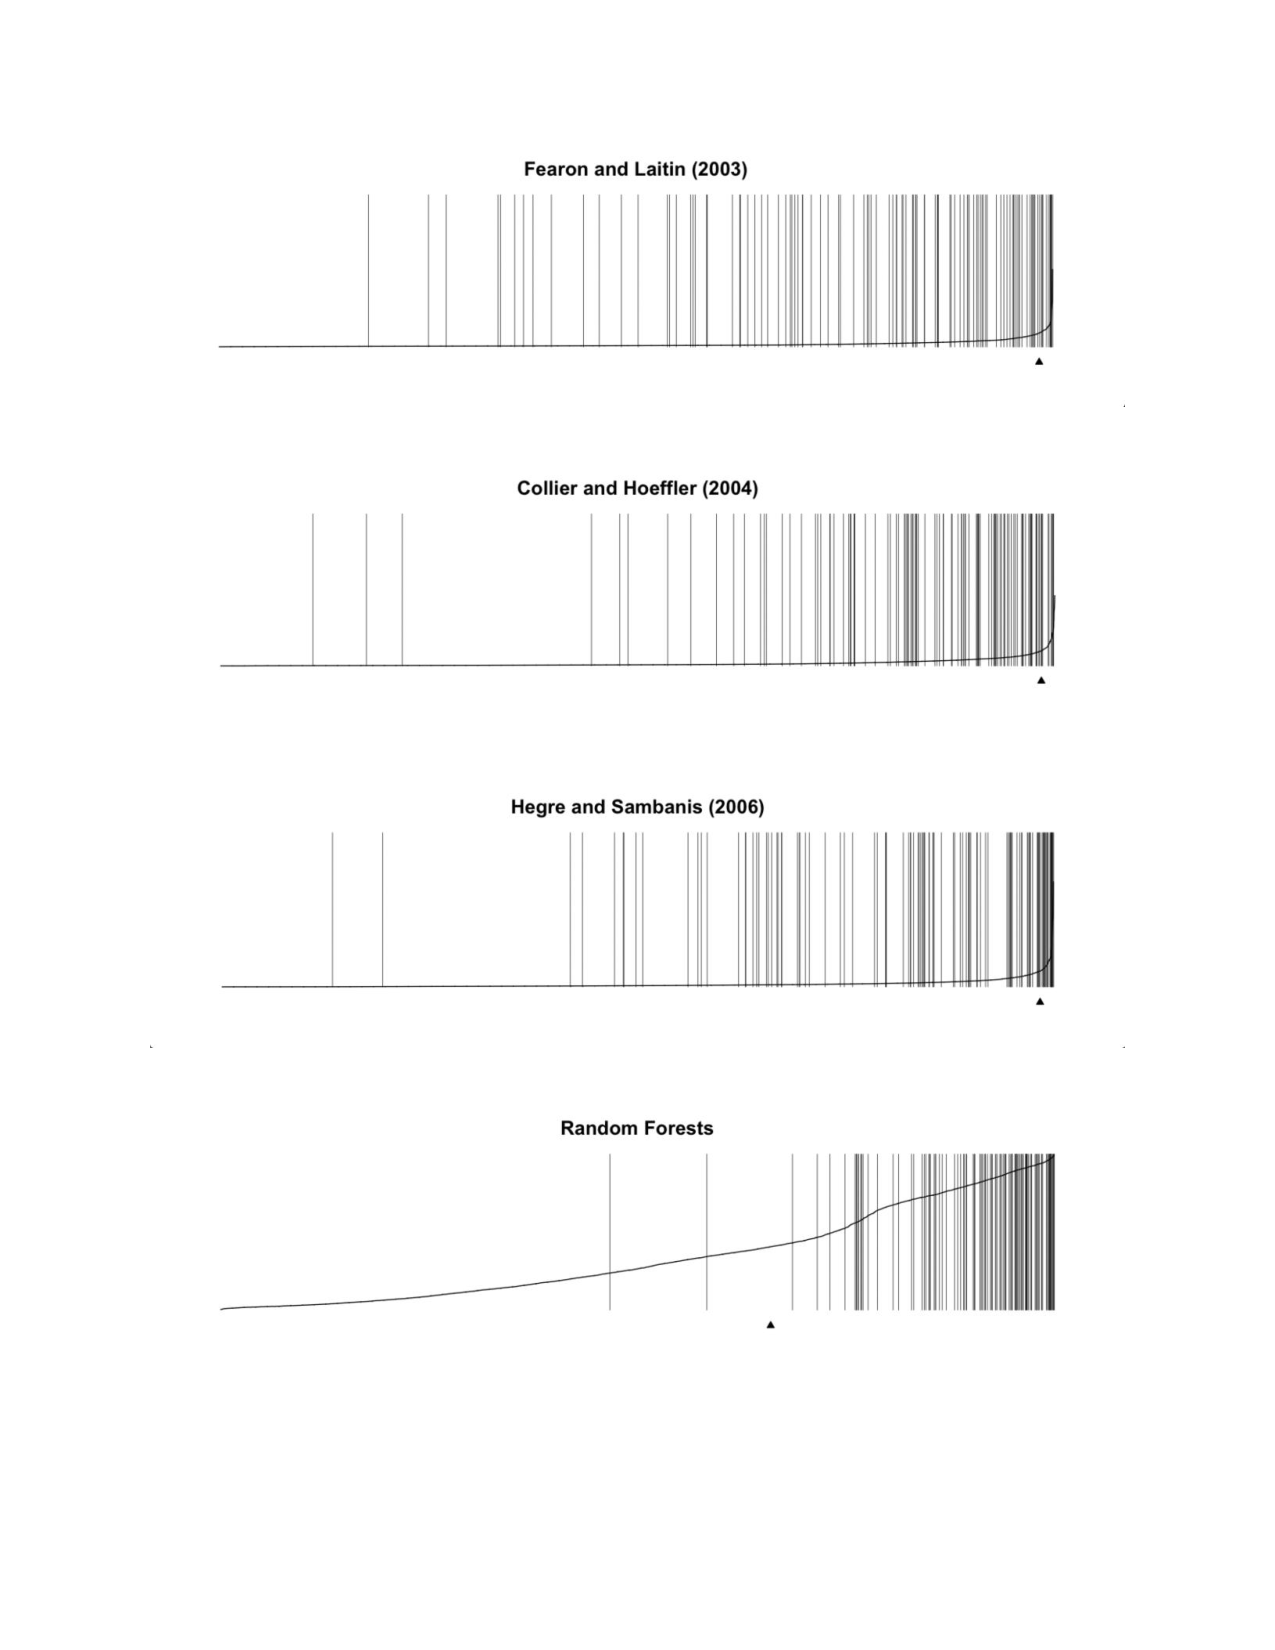
\includegraphics[width=1.3\textwidth]{Figures/figure1.pdf}}%
    \caption{Separation plot for all classifiers.}
\label{fig:separation}
\end{figure}

\begin{figure}[H]
    \makebox[\textwidth][c]{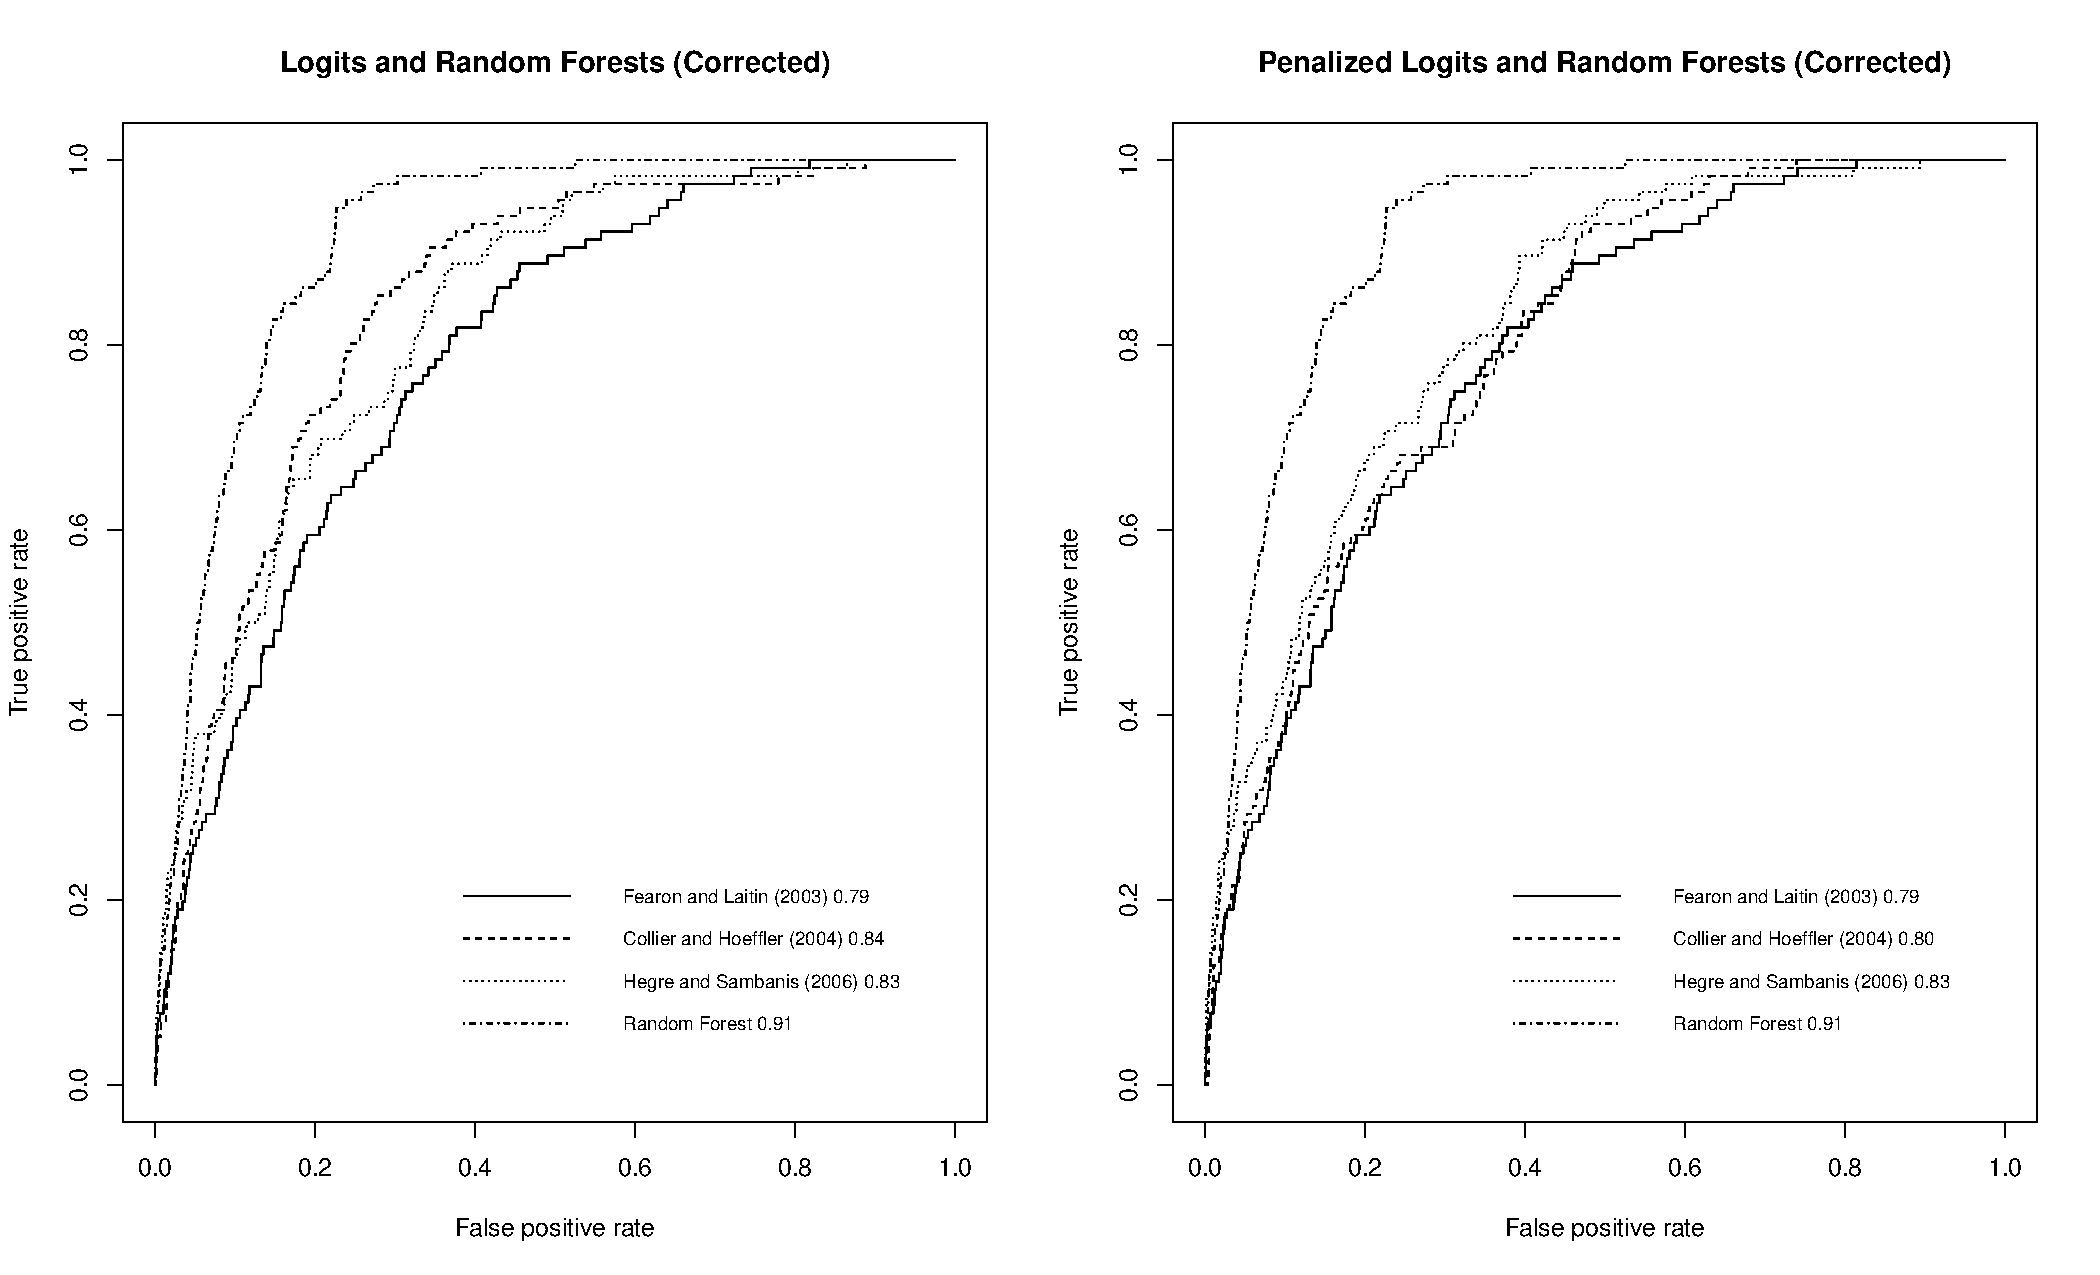
\includegraphics[width=1.4\textwidth]{Figures/figure2.pdf}}%
    \caption{ROC curves for all classifiers.}
\end{figure}



\section*{Part 2: Extension}
\subsection*{Introduction}
A central issue in the prediction setup proposed by Muchlinski et al. is the assumption that the onset of a civil war is a binary variable, such that civil war either occurred or did not occur in a given year. However, real-life civil war onset is rarely so discrete: skirmishes and widespread civil unrest often precede the onset of declared war. We questioned whether the results that Muchlinski et al. obtained might be dependent on the arbitrary cutoff for civil war on which their predictions depend.

To investigate this possibility, we examined whether continuous prediction of the degree of state violence would affect the relative predictive power of random forests and logistic regression models. Measuring the degree of unrest by the number of deaths per capita in a given year, we trained a random forest and a logistic regression model to examine their ability to predict the degree of violence.

We also examined whether methods improving on traditional random forests improve classifier results. We compared the performance of the random forest and logistic regression models to LightGBM, a faster variant of gradient boosting decision trees \citep{ke2017lightgbm}.

\subsection*{Methods}
The Uppsala Conflict Data Program (UCDP) measures the number of deaths per country due to several types of conflict. We used the number of deaths per country due to intrastate violence, which the UCDP defines as violence between a government and rebel troops without the involvement of foreign governments with troops, and internationalized intrastate violence, which the UCDP defines as violence between a government and rebel troops with some involvement of foreign governments with troops. We excluded deaths due to extrasystemic violence (between a state and a non-state outside its territory) and interstate violence as inapplicable to civil war. We then used the United Nations' popualtion data to determine the number of deaths per capita for each country in each year from 1989 to 2000.

\subsection*{Results}

\newpage

\renewcommand\refname{Bibliography}

\bibliographystyle{plainnat} % or try abbrvnat or unsrtnat
\bibliography{refs}
\end{document}
